\section{Interpolation \& Extrapolation}

\subsection{Polynom-Interpolation}

\begin{figure}[H]
    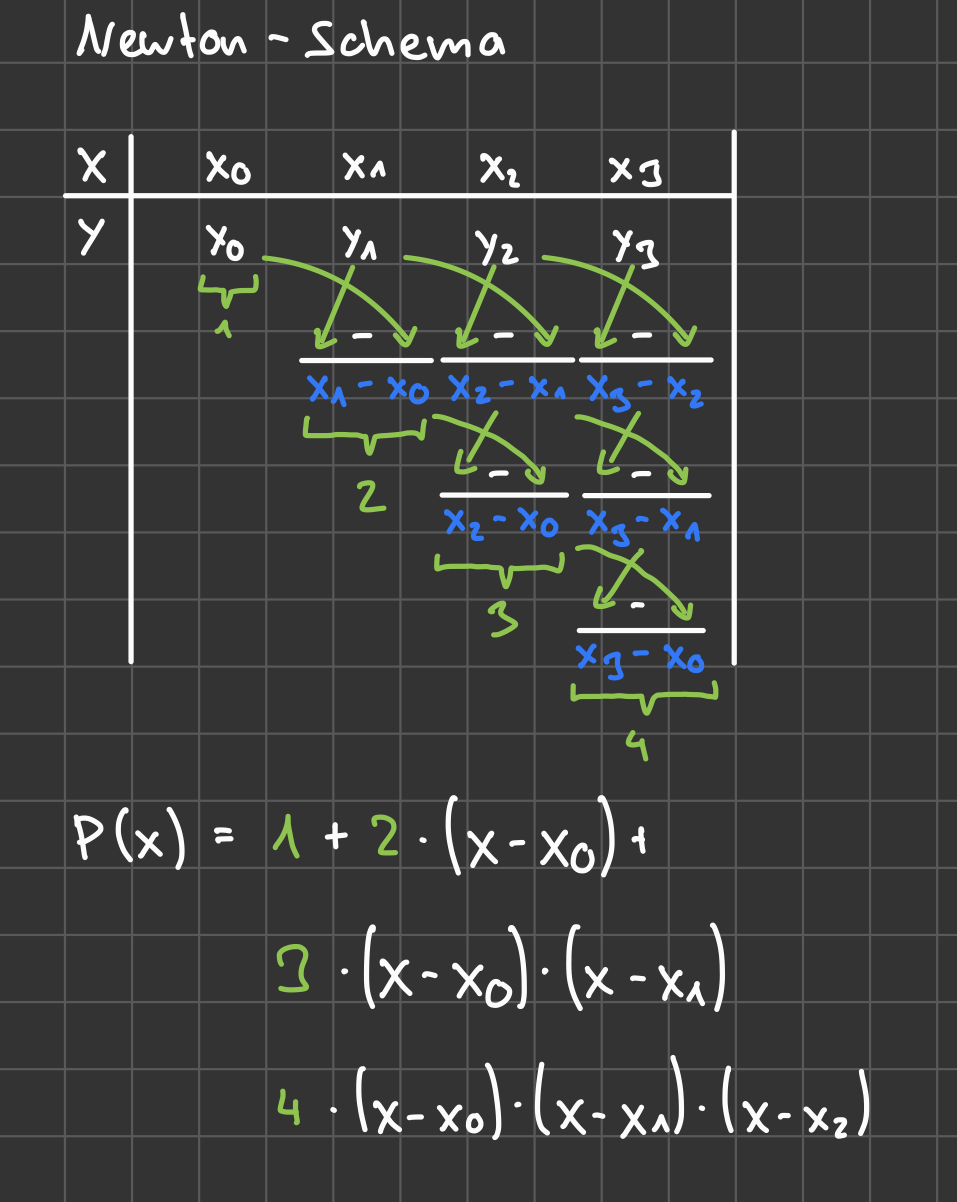
\includegraphics[height=8cm]{Newton_Schema}
\end{figure}

\subsection{Polynom-Extrapolation}

\begin{figure}[H]
    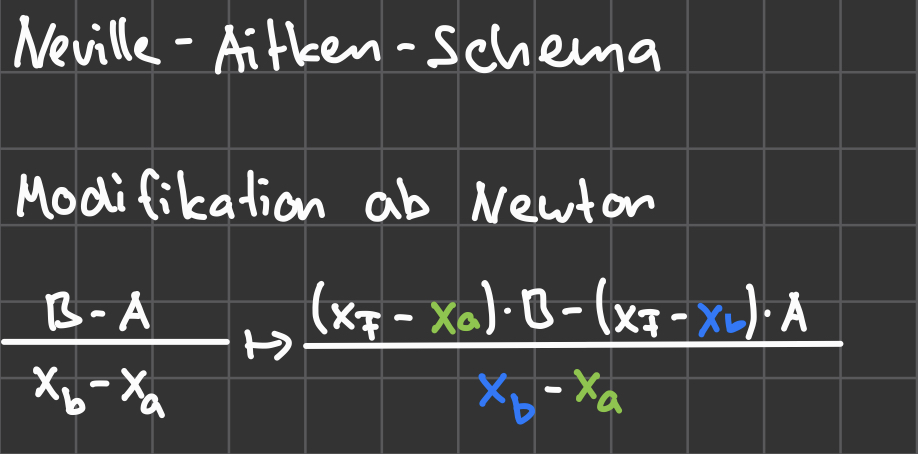
\includegraphics[width=8cm]{Neville_Aitken_Schema}
\end{figure}

\subsection{Regression}

\subsubsection{Lineare Regression}

\paragraph{LGLS in Matrix-Form}

\begin{displaymath}
    \vec{u} = \begin{bmatrix} m \\ q \end{bmatrix},
    \vec{x} = \begin{bmatrix} x_1 \\ \vdots \\x_N \end{bmatrix},
    \vec{y} = \begin{bmatrix} y_1 \\ \vdots \\y_N \end{bmatrix},
    A = \begin{bmatrix} x_1 & 1 \\ \vdots & \vdots \\ x_N & 1 \end{bmatrix}
\end{displaymath}

\begin{displaymath}
    A^T \cdot A \cdot \vec{u} = A^T \cdot \vec{y}
\end{displaymath}

\subsubsection{Exponentielle Regression}

Um die Regression zu finden, werden die Daten mittels
logarithmierung auf einen lineare Zusammenhang zurückgeführt.